\documentclass{article}
\newif\ifdvipdfm
\dvipdfmtrue
\ifdvipdfm
\newcommand{\mydriver}{dvipdfm}
\else
\newcommand{\mydriver}{dvips}
\fi

\usepackage[driver=\mydriver, top=1in, bottom=1in, left=1.25in, right=1.25in]{geometry}
\usepackage[\mydriver]{graphicx}

\begin{document}

\title{Rubik's Cube Virtual Data Model}
\author{Andrew Makousky}
\date{August 9, 2011}
\maketitle

Since a Rubik's Cube is a 3D object that can be looked at from several
different perspectives, there are also several different ways that a
Rubik's Cube model can be represented in the computer. Therefore, the
purpose of this document is to clarify the representation that is used
within this Rubik's Cube program.

First of all, we should start with which side will be regarded as the
front one. Take a Rubik's Cube and rotate it so that the white side
faces you and the red side is up. The green side should face right,
the blue side should face left, orange down, and yellow should be the
back side.

\begin{center}
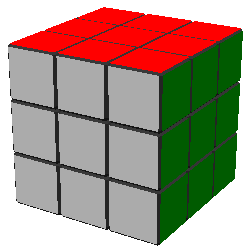
\includegraphics{image1}
\end{center}

A Rubik's Cube is composed of eight corner pieces, twelve edge pieces,
and six face pieces. When the Rubik's Cube is rotated, the corner and
edge pieces glide across the Rubik's Cube into their proper slots, but
the face pieces just rotate in place. Each corner piece can be rotated
to three different orientations in the same slot, and each edge piece
can be rotated to two different orientations in the same slot.

Lets start with the front face of the virtual model. When touching all
of the pieces on the front face, a fourth of the edges are touched and
half of the corners are touched. The first corner (index 0) will be
regarded as the top-right corner on the front face, and the next
corners will proceed counterclockwise. Then the numbering order for
the second set of corners is obtained by rotating the Rubik's Cube 180
degrees to look at the back as if it were the front, and continue
numbering in the same way.

\begin{center}
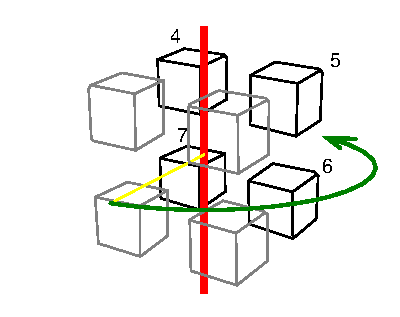
\includegraphics{image2}
\end{center}

In fact, the way the program renders the back corners is by rotating
the local rendering space around the z-axis as is shown in the figure
(the program uses the GL y-axis for the spatial z-axis), and then
proceeding according to which corner pieces are in which slots.

The corner rotations are a measure of how the corner colors would look
if you looked at the corner straight-on. The corner rotation states
have three possible values: 0, 1, or 2. The corner rotation state is a
measure of counterclockwise color rotation, zero being no rotation.

Now lets look at how the edges are represented. Cut out a strip of
paper that is as tall as the height of the Rubik's Cube and four times
as wide as a face on the Rubik's Cube. Then wrap this strip of paper
around the white, green, yellow, and blue sides of the Rubik's
Cube. When the paper is wrapped around the Rubik's Cube, draw a dot on
the center of each edge piece that the paper covers. Unwrap the paper
from the Rubik's Cube and lay it flat. For each face, draw a line that
connects the bottom dot to the right dot, and another line that
connects the right dot to the top dot.

\begin{center}
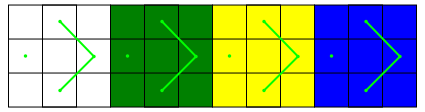
\includegraphics{image3}
\end{center}

Think of how the edges of faces are shared in the edge pieces. When
looking at the dots touched by the lines in this diagram, you can tell
that all twelve edge pieces are touched only once by such a dot. Also,
when you look down at the Rubik's Cube from the red face, you can see
that this ordering of faces proceeds counterclockwise.

Each edge piece in the Rubik's Cube program is formed by starting with
the bottom edge of a face, and filling then rotating counterclockwise
to the top edge of the face. Then the local coordinate space is
rotated to the next face to continue the process.

This document's central purpose was to introduce you to the data model
that is used within the Rubik's Cube program. As an introduction, it
told you summarized qualities of the data model that would otherwise
be difficult to obtain had you only been able to look at the source
code. Now that you know the general aspects of the data model used to
represent the Rubik's Cube in this program, you should understand that
the next steps are to look at the specifics contained within the
source code.

\end{document}
